%%%%%%%%%%%%%%%%%%%%%%%%%%%%%%%%%%%%%%%%%%%%%%%%%%%%%%%%%%%%%%%%%%%%%
%% This is a (brief) model paper using the achemso class
%% The document class accepts keyval options, which should include
%% the target journal and optionally the manuscript type.
%%%%%%%%%%%%%%%%%%%%%%%%%%%%%%%%%%%%%%%%%%%%%%%%%%%%%%%%%%%%%%%%%%%%%
\documentclass[journal=apchd5,manuscript=article]{achemso}
%%%%%%%%%%%%%%%%%%%%%%%%%%%%%%%%%%%%%%%%%%%%%%%%%%%%%%%%%%%%%%%%%%%%%
%% Place any additional packages needed here.  Only include packages
%% which are essential, to avoid problems later. Do NOT use any
%% packages which require e-TeX (for example etoolbox): the e-TeX
%% extensions are not currently available on the ACS conversion
%% servers.
%%%%%%%%%%%%%%%%%%%%%%%%%%%%%%%%%%%%%%%%%%%%%%%%%%%%%%%%%%%%%%%%%%%%%
\usepackage[version=3]{mhchem} % Formula subscripts using \ce{}
\usepackage[T1]{fontenc}       % Use modern font encodings
\usepackage{graphicx}
\usepackage{amsmath,amssymb}
%\usepackage{xcolor}
%\usepackage{wrapfig}
%\usepackage{multline}
%%%%%%%%%%%%%%%%%%%%%%%%%%%%%%%%%%%%%%%%%%%%%%%%%%%%%%%%%%%%%%%%%%%%%
%% If issues arise when submitting your manuscript, you may want to
%% un-comment the next line.  This provides information on the
%% version of every file you have used.
%%%%%%%%%%%%%%%%%%%%%%%%%%%%%%%%%%%%%%%%%%%%%%%%%%%%%%%%%%%%%%%%%%%%%
%%\listfiles

%%%%%%%%%%%%%%%%%%%%%%%%%%%%%%%%%%%%%%%%%%%%%%%%%%%%%%%%%%%%%%%%%%%%%
%% Place any additional macros here.  Please use \newcommand* where
%% possible, and avoid layout-changing macros (which are not used
%% when typesetting).
%%%%%%%%%%%%%%%%%%%%%%%%%%%%%%%%%%%%%%%%%%%%%%%%%%%%%%%%%%%%%%%%%%%%%
\newcommand*\mycommand[1]{\texttt{\emph{#1}}}

%%%%%%%%%%%%%%%%%%%%%%%%%%%%%%%%%%%%%%%%%%%%%%%%%%%%%%%%%%%%%%%%%%%%%
%% Meta-data block
%% ---------------
%% Each author should be given as a separate \author command.
%%
%% Corresponding authors should have an e-mail given after the author
%% name as an \email command. Phone and fax numbers can be given
%% using \phone and \fax, respectively; this information is optional.
%%
%% The affiliation of authors is given after the authors; each
%% \affiliation command applies to all preceding authors not already
%% assigned an affiliation.
%%
%% The affiliation takes an option argument for the short name.  This
%% will typically be something like "University of Somewhere".
%%
%% The \altaffiliation macro should be used for new address, etc.
%% On the other hand, \alsoaffiliation is used on a per author basis
%% when authors are associated with multiple institutions.
%%%%%%%%%%%%%%%%%%%%%%%%%%%%%%%%%%%%%%%%%%%%%%%%%%%%%%%%%%%%%%%%%%%%%
\author{Nicholas P. Montoni}
\author{Steven C. Quillin}
\author{Charles Cherqui}
\author{David J. Masiello}
\affiliation[Department of Chemistry, University of Washington]
{Department of Chemistry, University of Washington, Seattle, WA 98195}
\email{masiello@chem.washington.edu}
%\date{February 12, 2017}
%%%%%%%%%%%%%%%%%%%%%%%%%%%%%%%%%%%%%%%%%%%%%%%%%%%%%%%%%%%%%%%%%%%%%
%% The document title should be given as usual. Some journals require
%% a running title from the author: this should be supplied as an
%% optional argument to \title.
%%%%%%%%%%%%%%%%%%%%%%%%%%%%%%%%%%%%%%%%%%%%%%%%%%%%%%%%%%%%%%%%%%%%%
\title[]
    {Tunable Spectral Ordering of Magnetic Plasmon Resonances in Noble Metal Nanoclusters}
%%%%%%%%%%%%%%%%%%%%%%%%%%%%%%%%%%%%%%%%%%%%%%%%%%%%%%%%%%%%%%%%%%%%%
%% Some journals require a list of abbreviations or keywords to be
%% supplied. These should be set up here, and will be printed after
%% the title and author information, if needed.
%%%%%%%%%%%%%%%%%%%%%%%%%%%%%%%%%%%%%%%%%%%%%%%%%%%%%%%%%%%%%%%%%%%%%
%\abbreviations{MNP, LSPR, EELS}
\keywords{magnetic plasmons, plasmon metamolecules, plasmon oligomers, angle-resolved cathodoluminescence, retardation effects}

%%%%%%%%%%%%%%%%%%%%%%%%%%%%%%%%%%%%%%%%%%%%%%%%%%%%%%%%%%%%%%%%%%%%%
%% The manuscript does not need to include \maketitle, which is
%% executed automatically.
%%%%%%%%%%%%%%%%%%%%%%%%%%%%%%%%%%%%%%%%%%%%%%%%%%%%%%%%%%%%%%%%%%%%%
\begin{document}

%%%%%%%%%%%%%%%%%%%%%%%%%%%%%%%%%%%%%%%%%%%%%%%%%%%%%%%%%%%%%%%%%%%%%
%% The "tocentry" environment can be used to create an entry for the
%% graphical table of contents. It is given here as some journals
%% require that it is printed as part of the abstract page. It will
%% be automatically moved as appropriate.
%%%%%%%%%%%%%%%%%%%%%%%%%%%%%%%%%%%%%%%%%%%%%%%%%%%%%%%%%%%%%%%%%%%%%
\begin{tocentry}
\begin{centering}
\includegraphics[height=3.5cm]{toc.pdf}
%\caption{dffd}
\end{centering}
\ \\
For Table of Contents Use Only\\
``Tunable Spectral Ordering of Magnetic Plasmon Resonances in Noble Metal Nanoclusters''\\
Nicholas P. Montoni, Steven C. Quillin, Charles Cherqui, and David J. Masiello\\
Magnetic plasmon nanoclusters offer the ability to harness both the electric and magnetic components of light. If incorporated into plasmon-enhanced solar-light harvesting devices, such spectrally tunable nanostructures would more efficiently capture photons across the optical spectrum than traditional electric-plasmon-based architectures.
\end{tocentry}

%%%%%%%%%%%%%%%%%%%%%%%%%%%%%%%%%%%%%%%%%%%%%%%%%%%%%%%%%%%%%%%%%%%%%
%% The abstract environment will automatically gobble the contents
%% if an abstract is not used by the target journal.
%%%%%%%%%%%%%%%%%%%%%%%%%%%%%%%%%%%%%%%%%%%%%%%%%%%%%%%%%%%%%%%%%%%%%

\begin{abstract}
Experimental characterization of the optical and magnetic properties of noble metal nanoclusters has exposed a size regime in between single-ring and extended two-dimensional nanocluster networks where the behavior of magnetic plasmon resonances is not well understood. In this intermediate size regime, individual electric dipole plasmons on each nanoparticle within the cluster can hybridize into delocalized magnetic modes that couple to either the electric or magnetic field of light with seemingly arbitrary energy ordering. Here, using a coupled-dipole model that includes fully-retarded interactions between electric dipole plasmons, we show that magnetic plasmon resonance energies can be controllably tuned and even made to cross as a function of nanocluster size. Experimental confirmation of this prediction is challenging because optical selection rules dictate the simultaneous excitation of many spectrally-overlapping magnetic plasmon modes. However, based on analytic modeling and numerical simulation, we show that angle-resolved cathodoluminescence offers an approach to cleanly isolate these magnetic modes and observe the size-dependence of their spectrum. Not only does our work clarify the rich optical and magnetic behavior of noble metal nanoclusters in the intermediate-size regime, but it also suggests strategies to design negative-index plasmonic metamaterials with multiple tunable resonances in the visible spectrum.
\end{abstract}

%%%%%%%%%%%%%%%%%%%%%%%%%%%%%%%%%%%%%%%%%%%%%%%%%%%%%%%%%%%%%%%%%%%%%
%% Start the main part of the manuscript here.
%%%%%%%%%%%%%%%%%%%%%%%%%%%%%%%%%%%%%%%%%%%%%%%%%%%%%%%%%%%%%%%%%%%%
Plasmon oligomers, or metamolecules, are clusters of noble metal nanoparticles (MNPs) that exhibit anomalously strong magnetic character even though their individual nanoparticle building blocks do not. Known as magnetic plasmons, the collective cyclic oscillation of conduction-band electrons within each cluster has been shown to couple to and enhance the magnetic field of light and to hybridize with other clusters analogously to electric plasmons in individual MNPs \cite{Zhang2006,Zhang2007,NordHal2011,NordHal2012,Cherqui2014,Cherqui2016,Engheta2017}. Since their discovery in 2004 \cite{Shalaev2004}, such magnetic plasmon resonances have been the focus of a body of applied and fundamental research from negative index metamaterials\cite{Alu2006,Alu2008} to quantum tunneling \cite{Dionne2016}, sensing \cite{Yang2013,Chen17}, and Fano interferences \cite{Dionne2011,Liu2011,Cherqui2016,Wang17}. The magnetic properties of single oligomers, i.e., those clusters composed of only one ring of MNPs, are now well understood based upon quasistatic modeling, numerical simulation, and optical and electron-beam characterization \cite{Nord2006,Dionne2011,Dionne2016,Capolino2017}. Similar approaches have been employed to study toroidal dipole moments in nanoclusters \cite{Ogut2012toroidal,Yang2013,Zheludev2016,Wang17}. Infinitely extended two-dimensional networks of oligomers are also well understood theoretically \cite{Schatz2003,Weick2013}. However, recently, a disconnect between these extremes and methods has been discovered \cite{Cherqui2014,Engheta2017}, revealing a lack of understanding of how oligomer assemblies behave in the so-called intermediate size regime \cite{NordHal2011,NordHal2012,Cherqui2014,Qian2015,Cherqui2016,Engheta2017,Fakhraai2018,Scherer2018}.




Central to this disconnect is the question of when and how retardation effects matter. For example, in the case of the two oligomer cluster, the quasistatic approximation deviates from full-wave numerical electrodynamics simulations in that it predicts a different energy-ordering of the two magnetic plasmon resonances \cite{Cherqui2014}. It is well known that retardation effects can affect the electric plasmon energetics in single MNPs \cite{Gu2010}, dimers \cite{Oubre2004,vonPlessen2007}, and infinite chains and arrays \cite{Lucas1976,ARAVIND1981,Kottman2001,Schatz2003,NordHal2003,NordProdan2004,Rechbacher2003,Schatz2003,Royer2005,Abajo2008,Gomez2009,Chumanov2010,Pinchuk2016}. However, to date, no theoretical analysis has been reported on the role of retardation in the description of magnetic plasmon resonances, which are an intrinsically relativistic phenomenon. It is the purpose of this paper to show that the incorporation of retardation corrects the aforementioned disagreement between model and simulation which is pronounced in the intermediate-size regime, and further highlights the ability to tune the magnetic plasmon spectrum by changing the oligomer size. The latter observation is particularly important because it enables manipulation of the system's effective permittivity and permeability, thereby facilitating the design of future tunable optical metamaterials.



In the following, we present a coupled-dipole model to demonstrate the size-dependent evolution of the magnetic plasmons in intermediate-size $N$-ring oligomers, called $N$-mers, by including the effects of retardation in the mutual interaction of their underlying electric dipole plasmon resonances. Interestingly, as a function of size, we find that magnetic plasmon resonances switch their ordering in analogy to the way that electric plasmons in hybridized nanoparticles \cite{vonPlessen2007} and the giant electric and magnetic dipole plasmons of raspberry-like metamolecules \cite{Fakhraai2018} switch order. We further investigate the distinct radiative properties of these magnetic plasmons by computing the angle-resolved cathodoluminescence (CL) spectrum \cite{Hohenester2012,Hohenester2014,Coenen2011,CoPol2011,Polman2014}. CL is ideal over light scattering because the selection rules of the electron probe allow for the preferential excitation of specific magnetic responses, in distinction from light scattering where many broad higher-order electric responses are also excited. Building from the intuition gained, we finally analyze the size-dependent evolution of intermediate-size plasmonic nanoclusters similar to those characterized recently in Ref. \cite{Engheta2017}. We find that the spectral ordering depends not only on aggregate size but also upon morphology, offering a second handle to modify the spectrum. Such understanding may someday lead to advances in superlensing and electromagnetic cloaking at optical frequencies, as these applications benefit directly from the tunability of the system's electric and magnetic response \cite{Pendry03,Fang2005,Cai2007,Pinchuk07,Shalaev2008,Valentine2008,Ferrari09,Tian2018}.







\section*{Model Theory}
%%%%%%%%%%%%%%%%%%%%%%%%%%%%%%%%%%%%%%%%%%%%%%%%%%%%%%%%%%%%%%%%%%%%%%%
\begin{figure}
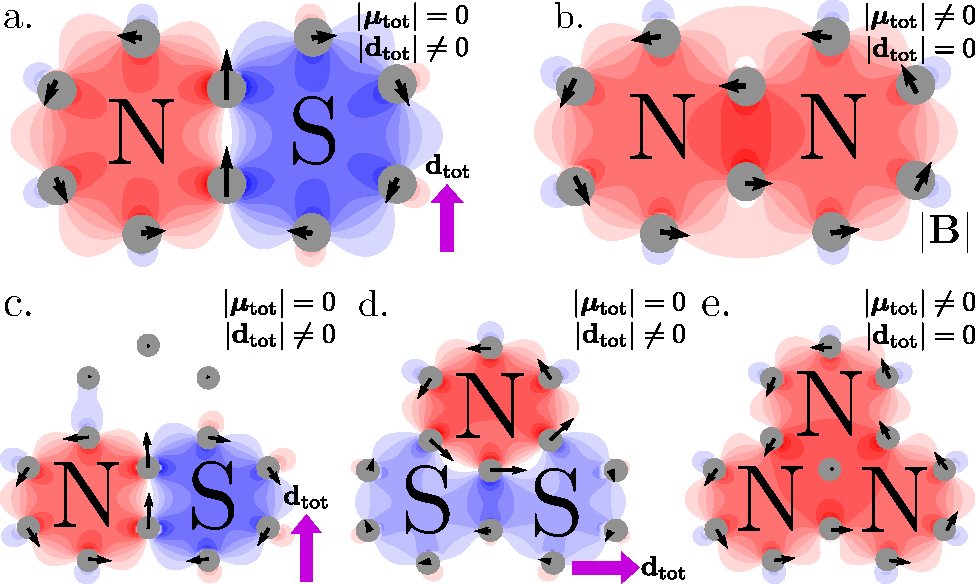
\includegraphics{fig1.pdf}
\caption{Signed magnetic field magnitude of the 2-mer's (a,b) and 3-mer's (c,d,e) magnetic plasmon resonances. Each system supports a number of closed-loop magnetic plasmons equal to the number of rings ($N$) in the oligomer. Magnetic plasmons that have a net electric dipole moment (a,c,d) show a node in their magnetic field and have no net magnetic dipole moment. Oppositely, the nodeless magnetic modes (b,e) possess a net magnetic dipole moment that interacts with the magnetic field of light.}
\label{field_plots}
\end{figure}
%%%%%%%%%%%%%%%%%%%%%%%%%%%%%%%%%%%%%%%%%%%%%%%%%%%%%%%%%%%%%%%%%%%%%%%
Fig. \ref{field_plots} displays two model oligomer systems, the 2-mer and 3-mer, comprising $n=10$ and $n=13$ silver nanospheres in analogy to the molecules naphthalene and phenalene. The electric plasmons of each MNP can be mapped onto a set of proxy harmonic oscillators as described in Ref. \cite{Cherqui2014,ARPC}. This approach forms the basis for modeling the collective magnetic plasmon responses described herein. In the limit where each nanoparticle, here restricted to a spherical geometry of radius $a$, possesses only an electric dipole plasmon resonance, the hybridized plasmon modes of the oligomer are the solutions of the equations of motion
\begin{equation}
\ddot{\textbf{q}}_i +\omega_{\textrm{sp}}^2\textbf{q}_i = \frac{e}{m_{\textrm{sp}}}\sum_{j\neq i}\textbf{E}_j(\textbf{r}_i),
\label{equation_of_motion}
\end{equation}
where $\omega_{\textrm{sp}}=\sqrt{\omega_{p}^2/(\varepsilon_\infty+2\varepsilon_b)-(\gamma/2)^2}$ is the complex Mie resonance frequency and $m_{\textrm{sp}} = e^2/\alpha_{\textrm{sp}}\omega_{\textrm{sp}}^2$ is the plasmon's effective mass defined in terms of the static polarizability $\alpha_{\textrm{sp}} = 3a^3/(\varepsilon_{\infty} + 2\varepsilon_b)$ \cite{Cherqui2014}. Here, $\omega_p$ is the metal's bulk plasma frequency, $\varepsilon_{\infty}$ and $\varepsilon_b$ are the high-frequency and background dielectric functions, and $\gamma$ is the sum of the Drude electron-ion scattering and radiation damping rates; the latter would stem from the addition of a radiation reaction force in the equations of motion of the form $\textbf{F}_{\textrm{rad},i}=(2e^2/3m_{\textrm{sp}}c^3)\dddot{\textbf{q}}_i$ \cite{Draine1993}. While these frictional forces are not explicitly included as velocity-dependent terms in the equations of motion, friction does contribute to the red-shift and linewidth broadening of the Mie resonance with increasing MNP size. The electric dipole moment $\textbf{d}_i = e\textbf{q}_i$ of each plasmon oscillator is restricted to lie in the plane of the oligomer (taken to be the $x-y$ plane) at position $\textbf{r}_i$, and $\textbf{E}_j(\textbf{r}_i)$ is the fully retarded electric field of the $j$th dipole evaluated at the position of the $i$th dipole. The electric field is defined by $\textbf{E}_j(\textbf{r}_i) = \boldsymbol{\Lambda}_{ij}\cdot\textbf{d}_j= \left\{\left(3\hat{\textbf{n}}_{ij}\hat{\textbf{n}}_{ij} - \textbf{1}_{ij}\right)\left({1}/{r_{ij}^3} - {ik}/{r_{ij}^2}\right) - \left(\hat{\textbf{n}}_{ij}\hat{\textbf{n}}_{ij} - \textbf{1}_{ij}\right)k^2/r_{ij}\right\}e^{ikr_{ij}}\cdot\textbf{d}_j/\varepsilon_b,$ where $\hat{\textbf{n}}_{ij}$ is the unit vector connecting two dipoles separated by distance $r_{ij}=|{\bf r}_i-{\bf r}_j|$ and $k=\sqrt{\varepsilon_b}\omega/c.$ The field is decomposed into three parts---the near- ($r_{ij}^{-3}$), intermediate- ($r_{ij}^{-2}$), and far-field ($r_{ij}^{-1}$)---which together include all dipolar retardation effects \cite{Purcell1973}. Interestingly, the latter term carries the opposite sign of the former two. As will be shown in the following, it is because of both the relative magnitude and sign of these terms as well as the oscillatory behavior of $e^{ikr_{ij}}$ that the interactions can change character and switch from energy-lowering to energy-raising. Since magnetic plasmons only involve the hybridization of $(x,y)$-oriented electric dipole plasmons that are orthogonal to the $z$-direction, only those $2n$ (of the $3n$) electric dipole plasmons in the $x-y$ plane are explicitly accounted for in Eq. (\ref{equation_of_motion}).



As described in the Methods Section, there are as many hybridized modes of each $N$-mer as there are electric dipole plasmons. Of these hybrid modes, some are electric and some are magnetic in character, with each $N$-mer studied here having $N$ magnetic plasmon resonances. Fig. \ref{field_plots} shows the magnetic plasmon modes of the 2-mer and 3-mer overlaid with their associated signed magnetic field magnitude. Each mode is named for its particular magnetic field distribution after the poles of a magnet, either all-North (aN) or North-South (NS). The top right-hand corner of each panel indicates the net electric or magnetic dipole moment magnitude. The black arrows denote the electric dipole plasmons on each MNP within each magnetic mode, while the magenta arrow indicates the mode's net electric dipole moment. In planar geometries, the magnetic dipole moments are always perpendicular to the in-plane electric dipole moments. As a result, they scatter light with different directionality as will be discussed.




\section*{Spectral Ordering of Magnetic Plasmon Modes in Intermediate-Size $N$-mers}
To determine the impact of incorporating retardation effects, it is first useful to consider the quasistatic limit. Here individual nanoparticle plasmon resonance frequencies ($\omega_{sp}$) are size-independent and the coupling strength depends only upon the scale $s_{ij} = r_{ij}/a$ and not upon the overall oligomer size. That is, if this ratio $s_{ij}$ of interparticle distance $r_{ij}$ to nanoparticle radius $a$ remains constant, the collective resonance frequencies do not change as the nanoparticles increase in size. This is evident by considering the $ka\ll 1$ limit of the interaction on the right-hand side of Eq. (\ref{equation_of_motion}),
\begin{equation}
\begin{aligned}
\lim_{ka \to 0}\frac{e}{m_{\textrm{sp}}}\textbf{E}_j(\textbf{r}_i) &= \frac{e^2}{m_{\textrm{sp}}}\boldsymbol{\Lambda}_{ij}\cdot{\bf q}_j\\ 
&= \frac{\omega_{\textrm{sp}}^2}{\varepsilon_b}\alpha_{\textrm{sp}}\frac{3\hat{\textbf{n}}_{ij}\hat{\textbf{n}}_{ij} - \textbf{1}_{ij}}{r_{ij}^3} \cdot \textbf{q}_j \\
&= \frac{\omega_{\textrm{sp}}^2}{\varepsilon_b} \left(\frac{3}{\varepsilon_{\infty}+2\varepsilon_b}\right)\frac{3\hat{\textbf{n}}_{ij}\hat{\textbf{n}}_{ij} - \textbf{1}_{ij}}{s_{ij}^3} \cdot \textbf{q}_j.
\end{aligned}
\label{quasistatic_coupling}
\end{equation}
Retardation effects, however, remove this invariance and introduce radius-dependence into both the Mie frequency and the electric field. Consequently, in the following, we choose the individual MNP radius $a$ as the independent variable. To define the oligomer geometry, we fix the nearest-neighbor distance to $3a,$ such that the distance between each MNP remains a fixed multiple of $a$ for any value of $a.$

%^ 3$a$ to investigate the effects of retardation upon the magnetic plasmon spectrum in intermediate-size $N$-mers.



%where $m_{\textrm{sp}}$ and $\alpha_{\textrm{sp}}$ are rewritten in terms of fundamental parameters for silver, i.e., $\varepsilon_{\infty} = 3.77$, $\hbar\gamma = 0.05$ eV, and $\hbar\omega_{p} = 9.1$ eV. 




%%%%%%%%%%%%%%%%%%%%%%%%%%%%%%%%%%%%%%%%%%%%%%%%%%%%%%%%%%%%%%%
\begin{figure}
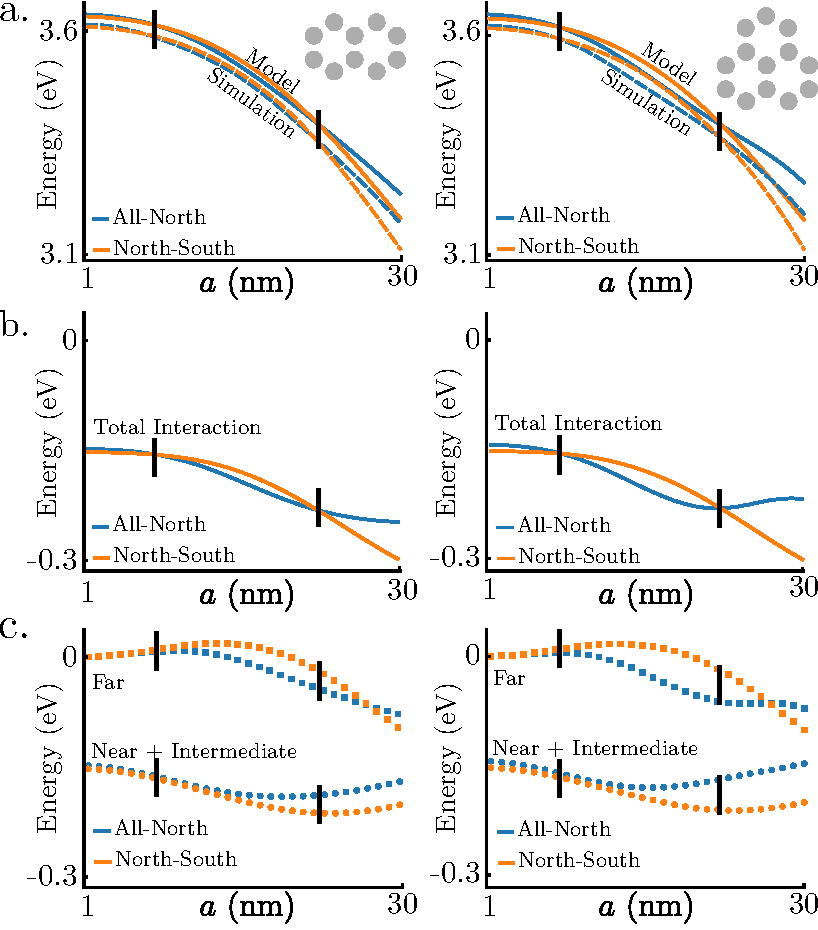
\includegraphics{fig2.pdf}
\caption{(a) Magnetic plasmon resonance energies and (b,c) electric dipole plasmon interaction energies of the 2-mer and 3-mer. For MNP radii $a\lesssim7$ nm, the magnetic modes are ordered as predicted by quasistatic theory, with the NS mode (orange) lower in energy than the aN mode (blue). This implies that for small oligomers, the quasistatic approximation is accurate. However, at sizes $7\lesssim a\lesssim20$ nm, the magnetic plasmon resonances switch spectral order. This is due to the relative strength of the far-field interaction (squares) in comparison to the near- and intermediate-field contributions (circles). Finally, for $a\gtrsim20$ nm, the magnetic plasmon resonances switch order again. Also shown in panel a are the corresponding simulated resonance energies of each magnetic plasmon mode (dashed lines), indicating excellent agreement with the presented coupled-dipole model.}
\label{scaling}
\end{figure}
%%%%%%%%%%%%%%%%%%%%%%%%%%%%%%%%%%%%%%%%%%%%%%%%%%%%%%%%%%%%%%%
Fig. \ref{scaling} shows the predicted magnetic plasmon resonance energies from both Eq. (\ref{equation_of_motion}) and full-wave numerical electrodynamics simulation of the 2-mer and 3-mer with increasing $a$ \cite{Hohenester2012}. At small $a$, the magnetic modes preserve the quasistatic ordering predicted in previous work \cite{Cherqui2014}, which is to be expected when the oligomer system fits within an optical wavelength and the near-field dominates the electric field. As the system size increases, the resonance energies decrease and cross at $a \approx 7$ nm, and once more at $a \approx 20$ nm. The second crossing recovers the same spectral ordering as at small sizes, which might lead to the erroneous conclusion that the quasistatic approximation is correct again. Rather, both crossings are due entirely to retardation effects as can be seen from the total interaction energy $U = -({1}/{2}) \sum_{ij} \textbf{d}_i \cdot \textbf{E}_j(\textbf{r}_i)$ between each pair of electric dipole plasmons within each magnetic plasmon mode. It is the inclusion of the far-field that causes the mode switching, as it carries the opposite sign of the near- and intermediate-field terms. Fig. \ref{scaling} shows the competition between these field components as well as their relative contributions to the total interaction energy. Inspection of Fig. \ref{scaling}c reveals that the crossing points occur where the splitting in the near- and intermediate-fields is equal and opposite to that of the far-field. Perhaps more interestingly, in any dielectric medium with $\varepsilon_b > 1$ the crossing points are shifted towards smaller scale due to wavelength contraction. This can be explained through the impact of dielectric medium upon the interaction energy $U,$ which increases with increasing $\varepsilon_b$ due mostly to the far-field term's dependence upon $k^2$ \cite{Elsayed2008}. While previous work has explored the oscillatory nature of hybridized electric dipole plasmon resonances and radiation damping as a function of separation in noble metal dimers \cite{vonPlessen2007}, our work shows that magnetic plasmon resonances also oscillate with interparticle separation and can be understood by analysis of the different contributions to the electric dipole-electric dipole interaction.


\section*{Radiative Properties of Intermediate-Size $N$-mers}
Only those magnetic resonances that have net electric or magnetic dipole moments will couple strongly to the radiation field. The magnetic dipole moment of the aN magnetic mode is perpendicular to the electric dipole moment(s) of the NS mode in both the 2-mer and 3-mer (see Fig. \ref{scattering}). This means that these modes radiate with different directionality. It has been predicted and shown experimentally that 1-mers scatter light anisotropically when both their magnetic and electric dipole moments are mutually excited, \cite{Dionne2011,Cherqui2016} as is evident in differential scattering spectra and radiation profiles. Both observations stem from the time-averaged differential power, \cite{jackson_classical_1999,schwinger1998classical}
\begin{equation}
\frac{dP({\bf x})}{d\Omega} = \frac{c}{8\pi}r^2\hat{\textbf{n}}\cdot\textrm{Re}\left[\sum_I\textbf{E}_I({\bf x}) \times \sum_{J}\textbf{B}_{J}^*({\bf x})\right]
\label{dp_field_1}
\end{equation}
observed at the point ${\bf x}=r\hat{\bf n},$ where $I,J=1,\ldots,N$ label the 1-mer unit cells within each $N$-mer. $\textbf{E}_I$ and $\textbf{B}_I$ are produced from the sum of effective electric ($\textbf{d}_I$) and magnetic ($\boldsymbol{\mu}_I$) dipole moments, assumed to be co-located at the center of the $I$th ring and oscillating in time as $e^{-i\omega t}$. In this approximation, the differential power becomes \cite{Alu2006}
\begin{equation}
\begin{split}
\frac{dP({\bf x})}{d\Omega} &= \frac{ck^4}{8\pi} \hat{\textbf{n}} \cdot \textrm{Re}\left[\left(\sum_{I} (\hat{\textbf{n}} \times \textbf{d}_I) \times \hat{\textbf{n}} - \hat{\textbf{n}} \times \boldsymbol{\mu}_I\right) \times \left(\sum_{J} \hat{\textbf{n}} \times \textbf{d}_J^* + (\hat{\textbf{n}} \times \boldsymbol{\mu}_J^*) \times \hat{\textbf{n}}\right)\right]\\
&= \frac{ck^4}{8\pi} \textrm{Re} \Bigg[ \sum_{IJ} \textbf{d}_I \cdot \textbf{d}_J^* - (\hat{\textbf{n}} \cdot \textbf{d}_I)(\hat{\textbf{n}} \cdot \textbf{d}_J^*) + \boldsymbol{\mu}_I \cdot \boldsymbol{\mu}_J^* - (\hat{\textbf{n}} \cdot \boldsymbol{\mu}_I)(\hat{\textbf{n}} \cdot \boldsymbol{\mu}_J^*) \\ 
&\hspace{2cm}+ \hat{\textbf{n}} \cdot (\textbf{d}_I \times \boldsymbol{\mu}_J^* + \textbf{d}_J^* \times \boldsymbol{\mu}_I) \Bigg].
\label{dp_dipoles_1}
\end{split}
\end{equation}
Notice that the first four terms involving $\bf d$ and $\boldsymbol\mu$ are due to the radiation produced by electric and magnetic dipoles, while the last term involving both is due to their interference. To build intuition, we fix the magnetic dipole moment $\boldsymbol{\mu}$ to point in the $z$-direction and the electric dipole $\textbf{d}$ to point in the $y$-direction for all $I,J.$ The effective electric and magnetic dipoles can be written in terms of their constituent dipoles as $\textbf{d}_I = \sum_i d_{I,i} \hat{\textbf{y}}$ and $\boldsymbol{\mu}_I = ({k}/{2})\sum_i\textbf{r}_i \times d_{I,i} \hat{\boldsymbol{\phi}}_i = ({knRd_{I,i}}/{2})\hat{\textbf{z}}$, where $R$ is the radius of the 1-mer ring consisting of $n$ nanoparticles, and $d_{I,i}$ is the electric dipole moment of the $i$th nanoparticle within the $I$th unit cell. For each $I$, all $d_{I,i}$ are equal.




%%%%%%%%%%%%%%%%%%%%%%%%%%%%%%%%%%%%%%%%%%%%%%%%%%%%%%%%%%%%%%%%%%
\begin{figure}
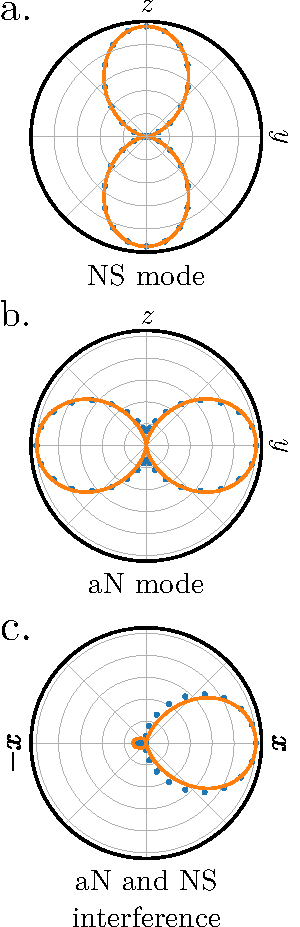
\includegraphics{fig3.pdf}
\caption{Differential radiative power profiles of the (a) NS and (b) aN magnetic plasmon resonances of the $N$-mer as well as (c) their interference as dictated by Eq. (\ref{dp_dipoles_1}). In all cases, the $N$-mer is oriented to lie in the $x-y$ plane so that the net electric dipole moment of the NS mode points along the $y$ axis and the net magnetic dipole moment of the aN mode points along the $z$ axis.}%For this geometry, the forward/backward directions refer to positive/negative $x$ direction.}
\label{scattering}
\end{figure}
%%%%%%%%%%%%%%%%%%%%%%%%%%%%%%%%%%%%%%%%%%%%%%%%%%%%%%%%%%%%%%%%%%
Fig. \ref{scattering} displays the differential scattering power profiles associated with the aN (a) and NS (b) magnetic plasmon resonances as well as their interference (c) for any $N$-mer with electric and magnetic dipoles oriented as described above. Since the aN mode has only a $z$-oriented magnetic dipole, its radiation pattern is orthogonal to that of the $y$-directed electric dipole of the NS mode. This means that asymmetry in the radiation pattern is due to the excitation of both modes. Thus, examination of the radiation directionality allows one to determine the net electric or magnetic dipole character. Such forward/backward scattering asymmetries have been predicted and demonstrated in metal-semiconductor core-shell nanoparticle assemblies, that similarly exploit the interference between electric and magnetic plasmons to direct light \cite{Kivshar2012}.


Recent studies have demonstrated the utility of angle-resolved CL spectroscopy to characterize plasmon resonances in noble metal nanoparticles\cite{Coenen2011,CoPol2011,Polman2014}. Using an electron microscope fitted with a parabolic mirror, emitted CL radiation can be collected across a large portion of the backward scattering hemisphere\cite{Coenen2011,CoPol2011,Polman2014}. Here we show that with the selection rules imposed by the location of the electron beam and the specific directionality of light emission, the size-dependent spectral order of the $N$-mers' magnetic plasmon modes can be observed in angle-resolved CL spectra. 


%More specifically, based upon the selection rules imposed by the electron beam and the directionality of CL radiation, it is possible to distinguish the magnetic modes and their spectral ordering as a function of size.



%%%%%%%%%%%%%%%%%%%%%%%%%%%%%%%%%%%%%%%%%%%%%%%%%%%%%%%%%%%%%%%%%%%%%
\begin{figure}
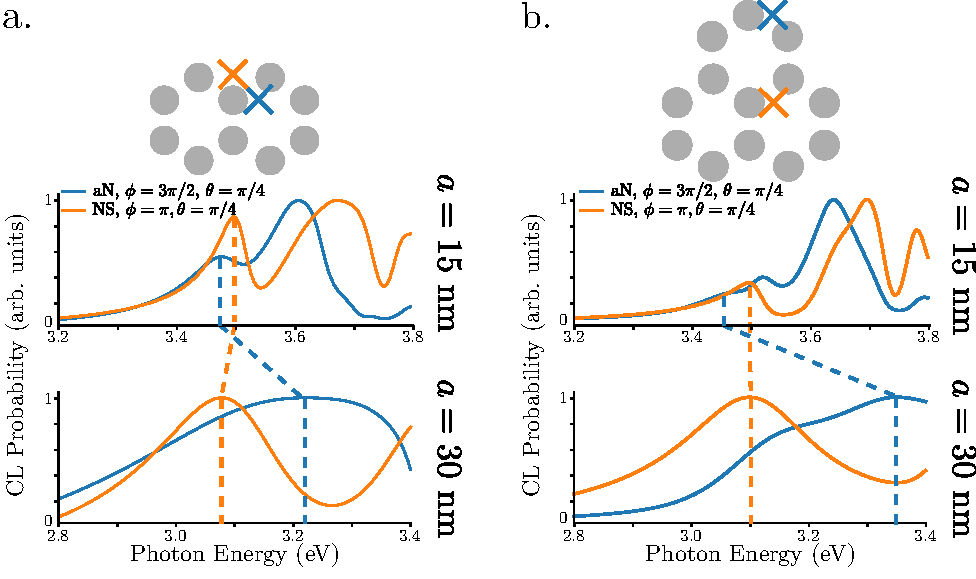
\includegraphics{fig4.pdf}
\caption{Angle-resolved cathodoluminescence spectra of the 2-mer (a) and 3-mer (b). Choosing the electron beam positions ($\times$) together with the light collection angles indicated allows the individual magnetic plasmon resonances and their size-dependent spectral switching to be observed. Simulated CL spectra with $a=15$ nm show the aN modes lower in energy than the NS modes, as predicted. With $a= 30$ nm, the modes switch in accordance with the presented coupled-dipole model. Spectral peaks located at higher energies correspond to higher-order non-magnetic plasmon modes that are not explicitly studied here.}
\label{CL_2mer_3mer}
\end{figure}
%%%%%%%%%%%%%%%%%%%%%%%%%%%%%%%%%%%%%%%%%%%%%%%%%%%%%%%%%%%%%%%%%%%%%
The previous section built up intuition on the directionality of light scattered by the magnetic modes of the 2-mer and 3-mer. This intuition informs the particular angles at which to collect CL spectra. Fig. \ref{CL_2mer_3mer} shows simulated point angle-resolved CL spectra of the 2-mer and 3-mer, with the electron beam position chosen so as to excite the aN (blue) and NS (orange) modes. Note however, due to the symmetry of the oligomers, the blue electron beam position excites not only the aN mode, but also weakly the NS mode. Since the radiation profile of the aN mode is orthogonal to that of the NS mode, it is possible to distinguish them by analyzing the angular distribution of emitted CL radiation, even though their splitting is $<0.05$ eV. The angle-resolved CL spectra at two such angles are reported in Fig. \ref{CL_2mer_3mer}. These simulated spectra confirm the predictions of the model displayed in Fig. \ref{scaling}; specifically, between $a = 15 - 30$ nm, the aN and NS modes switch spectral order. The simulation also shows mode switching at $a\approx7$ nm, however, the splitting energies are too small to be experimentally detectable with conventional CL. Nevertheless, experimental confirmation of the secondary mode splitting is possible, and would verify both our analytical and numerical predictions.










\section*{Magnetic Plasmon Resonances in Hexagonally-Packed Nanoclusters}
Ref. \cite{Engheta2017} synthesizes, fabricates, and optically characterizes hexagonally-packed nanoclusters composed of gold nanoparticles in the intermediate size regime, between few particle nanoclusters and infinite arrays. Here, we apply our analytical modeling and numerical simulation to investigate the behavior of magnetic plasmon resonances in silver nanoclusters of the same geometry as a function of size, with an eye toward engineering magnetic resonances at particular resonance energies. Such tunability may be important in the design of future negative index materials with spectral tunability. Specifically, we consider hexagonally packed clusters composed of 13, 19, and 31 MNPs displayed in Fig. \ref{kagan_fields} as well as the insets of Fig. \ref{kagan_eigen}.




%%%%%%%%%%%%%%%%%%%%%%%%%%%%%%%%%%%%%%%%%%%%%%%%%%%%%%%%%%%%%%%%%
\begin{figure}
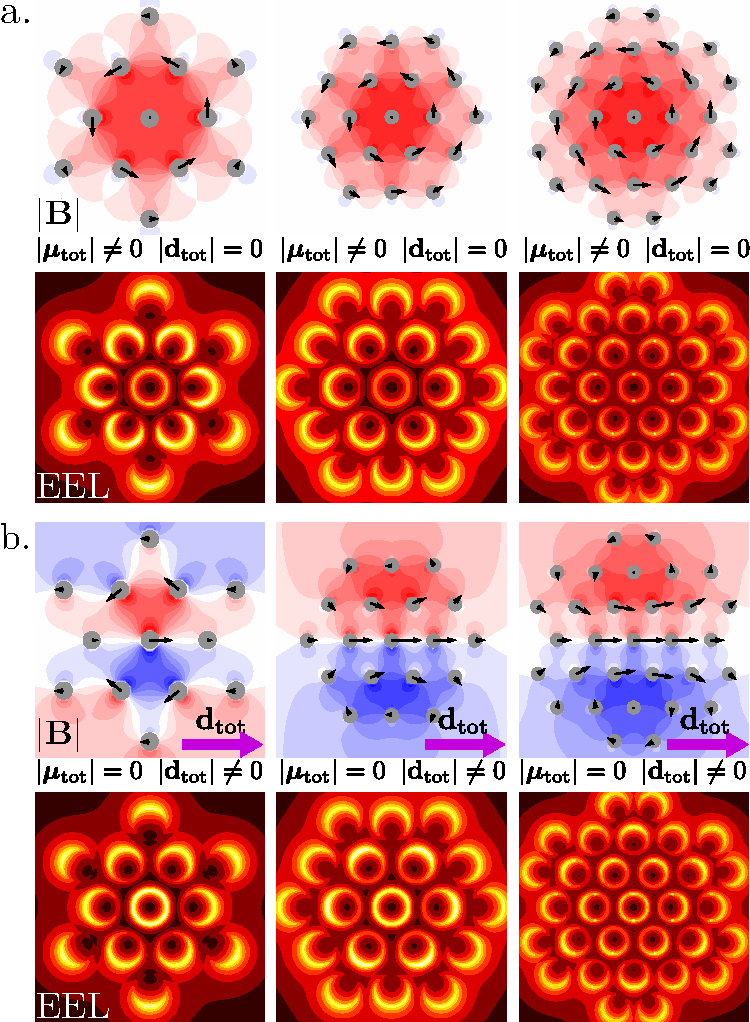
\includegraphics{fig5.pdf}
\caption{Signed magnetic field magnitudes and EEL mode maps of the aN (a) and NS (b) magnetic plasmon modes of 13-, 19-, and 31-particle nanoclusters. The clusters are based on those characterized in Ref. \cite{Engheta2017}, but are composed of silver. The magnetic fields are computed from the coupled-dipole model, while EEL mode maps result from simulation. As with the $N$-mers, only the NS modes have a net electric dipole moment indicated by the magenta arrow. The EEL mode maps indicate those regions in space where it is most probable to excite each magnetic plasmon.}
\label{kagan_fields}
\end{figure}
%%%%%%%%%%%%%%%%%%%%%%%%%%%%%%%%%%%%%%%%%%%%%%%%%%%%%%%%%%%%%%%%%
Fig. \ref{kagan_fields} displays the signed magnetic field magnitude of the aN (panel a) and NS (panel b) magnetic plasmon resonances of the 13-, 19-, and 31-particle nanoclusters. The black arrows denote the electric dipole moments of the individual MNPs within each magnetic plasmon mode, the magenta arrows denote the net electric dipole moment of the nanocluster, and the background color denotes the strength of the associated magnetic field. The net electric or magnetic dipole magnitude is denoted below each panel. The lower rows of panels a and b display the energy-filtered electron energy-loss (EEL) profiles of these modes. It is important to note that each aN mode is weakly excitable from the middle MNP (as indicated by the low EEL probability surrounding it), while the NS mode is strongly excitable from the same location (as indicated by the high EEL probability surrounding it). In all cases, the NS mode is doubly degenerate as would be true of any structure with sixfold symmetry. In analogy to the oligomers, these magnetic modes are chosen because they are the simplest (i.e., lowest order) and their radiation patterns are spatially orthogonal. 



%%%%%%%%%%%%%%%%%%%%%%%%%%%%%%%%%%%%%%%%%%%%%%%%%%%%%%%%%%%%%%%%%%%%%%
\begin{figure}
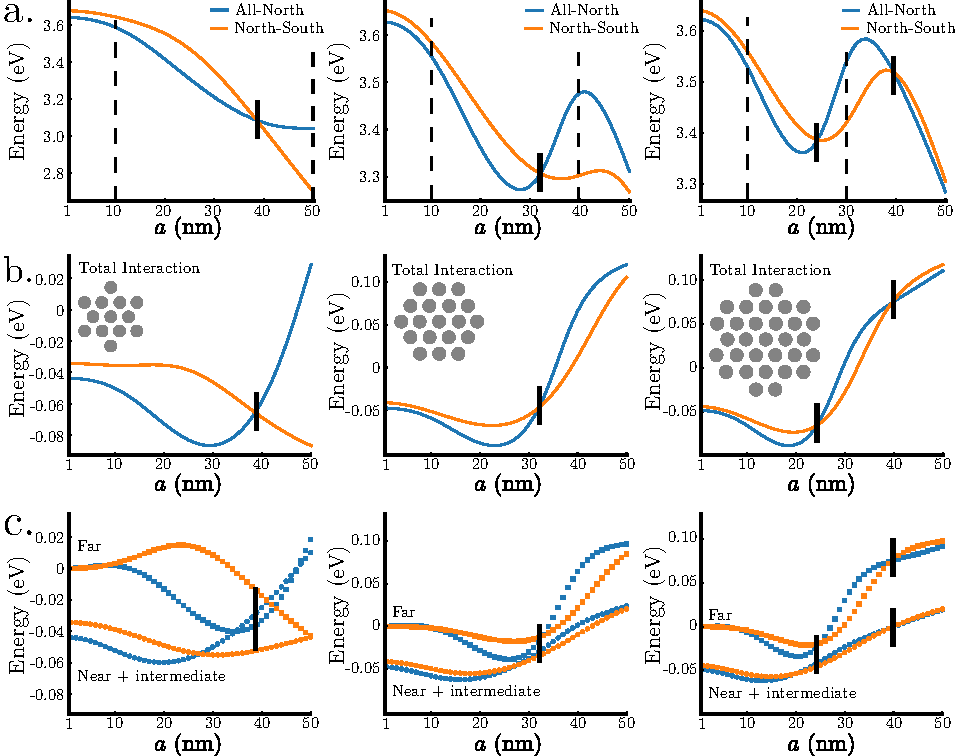
\includegraphics{fig6.pdf}
\caption{Magnetic plasmon resonance energies (a) and electric-dipole interaction energies (b,c) of 13-, 19-, and 31-particle nanoclusters similar to those characterized in Ref. \cite{Engheta2017}, but composed of silver. Due to the geometrical differences between these nanoclusters and the $N$-mers, the aN modes remain lowest in energy at small MNP radii $a$. However, as $a$ increases, one or even multiple magnetic plasmon resonance crossings become possible for the same reasons described earlier for the $N$-mers.}
\label{kagan_eigen}
\end{figure}
%%%%%%%%%%%%%%%%%%%%%%%%%%%%%%%%%%%%%%%%%%%%%%%%%%%%%%%%%%%%%%%%%%%%%%
Fig. \ref{kagan_eigen} displays the evolution of the aN and NS magnetic resonances with size $a$ as dictated by the coupled-dipole model. Here the size-dependent behavior of the nanocluster resonances is different due to the hexagonal packing as opposed to the open-ring structure of the $N$-mer. Nevertheless, the model is capable of predicting the magnetic spectrum. Most surprising is the oscillatory behavior of the nanoclusters' magnetic resonances with size as opposed to the expected monotonic red-shifting of those of the $N$-mer (see Fig. \ref{scaling}). Panels b and c display the total interaction energy $U$, and its near-, intermediate-, and far-field contributions, showing that this oscillatory behavior is due to retardation effects through the $e^{ikr_{ij}}$ factor in the electric field of each electric dipole.



%This is contrary to intuition where increasing size causes monotonic redshifting. However this oscillatory behavior is not so unexpected; separating a MNP dimer causes its hybridized electric plasmon resonance frequencies to oscillate from bonding to anti-bonding and back\cite{vonPlessen2007}. In these nanoclusters, ARCL and patterns spectra provide a means to demonstrate this oscillation.






%%%%%%%%%%%%%%%%%%%%%%%%%%%%%%%%%%%%%%%%%%%%%%%%%%%%%%%%%%%%%%%%%%%%%%
\begin{figure}
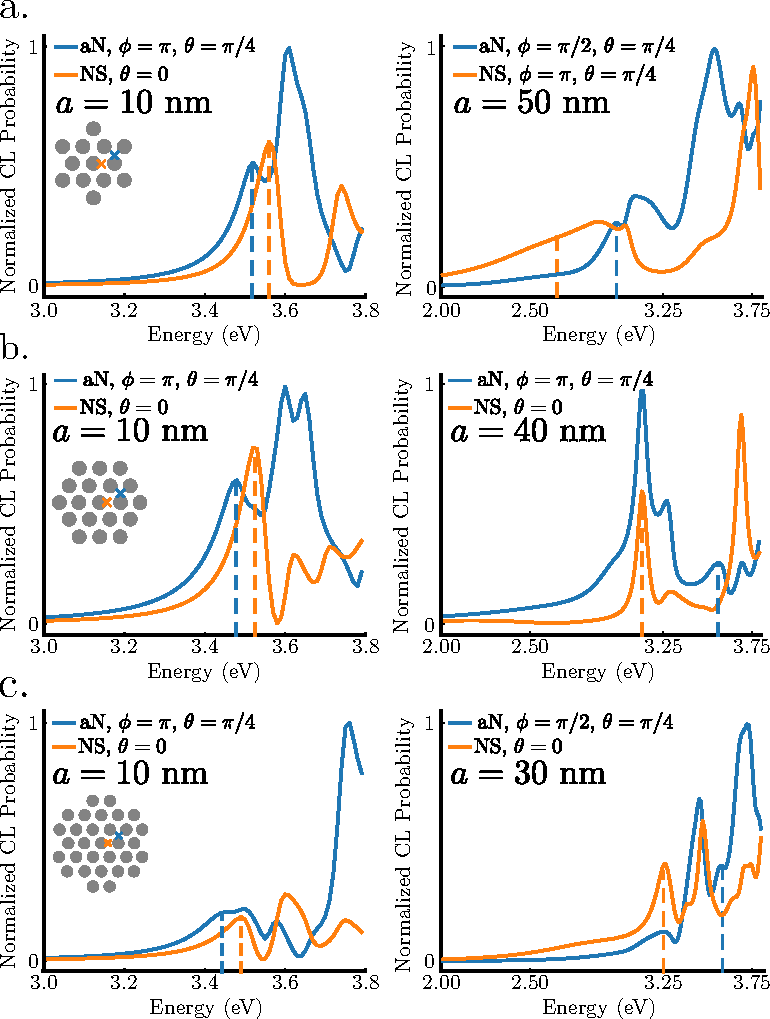
\includegraphics{fig7.pdf}
\caption{Simulated angle-resolved cathodoluminescence spectra of the (a) 13-, (b) 19-, and (c) 31-particle nanoclusters from Ref. \cite{Engheta2017}, but composed of silver. Blue (orange) spectra are acquired at the beam positions marked with a blue (orange) $\times$ to preferentially excite the aN ($x$-polarized NS) mode. The dashed lines in each spectrum indicate the resonance locations of the aN (blue) and NS (orange) modes. Each panel also displays the light collection angles associated with each spectrum. Again, all unlabeled resonance peaks correspond to higher-order plasmon modes of either electric or magnetic character, which are not studied herein.}
\label{kagan_CL}
\end{figure}
%%%%%%%%%%%%%%%%%%%%%%%%%%%%%%%%%%%%%%%%%%%%%%%%%%%%%%%%%%%%%%%%%%%%%%
Fig. \ref{kagan_CL} shows simulated angle-resolved CL spectra for the 13-, 19-, and 31-particle nanoclusters acquired at the two indicated beam positions and collection angles. Inspection of the EEL maps of the NS and aN magnetic resonances in Fig. \ref{kagan_fields} indicates the optimal electron beam positions to excite each magnetic plasmon mode, i.e., those positions with highest EEL probability. In particular, the NS mode (Fig. \ref{kagan_fields}b) is most easily excited near the central MNP, while the aN mode (Fig. \ref{kagan_fields}a) is more easily excited from the outer MNPs surrounding the central MNP. Upon selecting the appropriate excitation location, the radiative profile of each mode further helps identify the two magnetic resonances of interest. Because the aN mode radiates strongly in the $x-y$ plane, and weakly in the $z$-direction, it is detectable at angles between $0 < \theta \leq \pi/2$ for all $\phi$. Alternatively, by alignment with the $x$-axis, the NS mode is detectable at angles between $0 \leq \theta < \pi/2$ and $0<\phi<\pi,$ and $\pi<\phi<2\pi.$ The aN beam position also weakly excites the degenerate NS modes, meaning the corresponding CL spectrum will provide a secondary signature of the spectral location of that mode. This fact is evident in multiple simulated CL spectra displayed in Figs. \ref{CL_2mer_3mer} and \ref{kagan_CL}, demonstrating again the ability of angle-resolved CL to distinguish between resonances split by $\lesssim0.05$ eV. It should be noted that synthesis methods like those employed in Ref. \cite{Engheta2017} result in nearly spherical nanoparticles. However, if electron-beam lithography is used, the resulting nanoparticles will be more disklike in shape. This will have the effect of contributing a net redshift to the collective, in-plane plasmonic modes of the nanocluster \cite{Noguez}, while having negligible impact on the qualitative behavior of their energy ordering.




\section*{Conclusion}
In conclusion, we have presented a coupled-dipole model of MNP oligomers and hexagonally-packed nanoclusters that includes the effects of retardation and use it to show that the spectral ordering of their magnetic plasmon resonances can be controllably tuned as a function of cluster size and morphology. Full-wave numerical simulation is used to confirm the prediction that magnetic plasmon resonances can even be made to switch energy order, offering a relatively facile way to modify the system's magnetic responses in an experiment. The presented analysis is especially important in elucidating the intermediate-size regime in between individual single-ring and extended two-dimensional nanocluster networks, where retardation effects can significantly modify the spectrum. We further study the angular-dependence of the power emitted from the nanoclusters and demonstrate that the aN and NS magnetic plasmon modes, as well as their size- and morphology-dependent spectral order, can be detected in angle-resolved CL. Taken together, our work not only clarifies the rich optical and magnetic behavior of noble metal nanoclusters in the intermediate-size regime, but also suggests a strategy to design negative-index plasmonic metamaterials with multiple tunable resonances in the visible spectrum.





\section*{Methods}
\noindent{\it{Coupled-dipole model.}} Refs. \cite{Cherqui2014,ARPC} describe how to map the solutions of Maxwell's equations for electric plasmon resonances onto mechanical oscillators with effective masses. Based on this approach, the resulting Hamiltonian for a system of $n$ frictionless coupled oscillators is
\begin{equation}
H = \sum_{i}\frac{\textbf{p}_i^2}{2m_{\textrm{sp}}}+\frac{1}{2}m_{\textrm{sp}}\omega_{\textrm{sp}}^2\textbf{q}_i^2 - \frac{e}{2}\sum_{ij (i\neq j)}\textbf{q}_i\cdot\textbf{E}_j(\textbf{r}_i),
\label{hammy}
\end{equation}
where ${\bf q}_i$ and $\textbf{p}_i$ are the coordinate and momentum of the $i$th plasmon oscillator located at ${\bf r}_i$ with effective mass $m_{\textrm{sp}}$ and resonance frequency $\omega_{\textrm{sp}}$, defined previously. $\textbf{E}_j(\textbf{r}_i)$ is the full electric dipole field. The resulting equations of motion are,
\begin{equation}
\ddot{\textbf{q}}_i = -\omega_{\textrm{sp}}^2\textbf{q}_i + \frac{e}{m_{\textrm{sp}}}\sum_{j\neq i}\textbf{E}_j(\textbf{r}_i,\omega)
\label{equation_of_motion_again}
\end{equation}
which is Eq. (\ref{equation_of_motion}). Assuming sinusoidal oscillation in time and rewriting the electric field in terms of the plasmon coordinate results in the equations of motion
\begin{equation}
(\omega_{\textrm{sp}}^2-\omega^2)\textbf{q}_i -\frac{e^2}{m_\textrm{sp}}\sum_{j\neq i}\boldsymbol{\Lambda}_{ij}(\omega)\cdot\textbf{q}_j = 0.
\label{fourier_eom}
\end{equation}
It is this system of equations for the plasmon oscillator coordinates that we solve to determine the magnetic plasmon resonances. Considering $n=2$ identical, coupled, collinear oscillators as an example and projecting out the directional-dependence, Eq. (\ref{fourier_eom}) becomes
\begin{equation}
\begin{split}
(\omega_{\textrm{sp}}^2-\omega^2)q_1 -g_{12}(\omega)q_2 &= 0\\
(\omega_{\textrm{sp}}^2-\omega^2)q_2 -g_{12}(\omega)q_1 &= 0,
\label{fourier_eom_12}
\end{split}
\end{equation}
or, equivalently,
\begin{equation}
\begin{bmatrix}
\omega_{\textrm{sp}}^2-\omega^2 & -g_{12}(\omega)\\
-g_{12}(\omega) & \omega_{\textrm{sp}}^2-\omega^2
\end{bmatrix}
\begin{bmatrix}
q_1\\
q_2
\end{bmatrix}
=
\begin{bmatrix}
0\\
0
\end{bmatrix}.
\label{eom_matrix}
\end{equation}
where $g_{12}=-2e^2[r_{12}^{-3} - ikr_{12}^{-2}]e^{ikr_{12}}/\varepsilon_bm_{\textrm{sp}}.$ Note that the far-field contribution to $g_{12}$ vanishes here due to the assumed collinear arrangement of the dipoles. Solution of this system produces the hybridized plasmon resonance frequencies and modes of the dimer. Specifically, they are
\begin{equation}
\omega_{\pm} = \sqrt{\omega_{\textrm{sp}}^2 \pm g_{12}(\omega)}
\label{eigenvalues}
\end{equation}
and
\begin{equation}
q_{\pm} = \frac{1}{\sqrt{2}}\left(q_1 \pm q_2\right).
\label{eigenvectors}
\end{equation}
Note that the coupling term $g_{12}(\omega)$ is frequency dependent, meaning that the eigenvalue problem must be solved iteratively until convergence. The magnetic plasmon resonances described herein are obtained as a straightforward extension of this dimer example.




\noindent{\it{Simulation details.}} Optical and electron beam simulations were performed using the MNPBEM package \cite{Hohenester2012,Hohenester2014}. Each spherical nanoparticle was discretized into 144 surface elements, each assigned the following Drude model parameters for silver: $\varepsilon_{\infty} = 3.77$, $\hbar\gamma = 0.05$ eV, and $\hbar\omega_{p} = 9.15$ eV. The electron kinetic energy was chosen to be 200 keV and all calculations were performed in vacuum, i.e., $\varepsilon_{b}=1.$ The angle-resolved CL spectra were computed using standard functions within MNPBEM together with numerical angular integration through $\pm25^\circ$ about the angles $(\theta,\phi)$ indicated in the figures.


\begin{acknowledgement}
This work was supported by the U.S. Department of Energy Basic Energy Sciences under award number DE-SC0018040 (D.J.M.) and by the State of Washington through the University of Washington Clean Energy Institute and via funding from the Washington Research Foundation (N.P.M.). This work was facilitated through the use of advanced computational, storage, and networking infrastructure provided by the Hyak supercomputer system and funded by the STF at the University of Washington. N.P.M. would like to thank Dr. Niket Thakkar and Harrison Goldwyn for helpful discussions and advice.
\end{acknowledgement}

%%%%%%%%%%%%%%%%%%%%%%%%%%%%%%%%%%%%%%%%%%%%%%%%%%%%%%%%%%%%%%%%%%%%%
%% The appropriate \bibliography command should be placed here.
%% Notice that the class file automatically sets \bibliographystyle
%% and also names the section correctly.
%%%%%%%%%%%%%%%%%%%%%%%%%%%%%%%%%%%%%%%%%%%%%%%%%%%%%%%%%%%%%%%%%%%%%
\bibliography{references}
\end{document}


%While good for theoretical studies of system properties, scale is not tunable in real time, meaning these properties can't be easily measured. Recent research has focused heavily on finding controllable and reversible ways to manipulate the aggregation scheme of a metal nanoparticle array using tools like DNA, polymers, and stretchable embedding media\cite{Yang2016,Ginger2017,NaLiu2017,DanLuo2009}. We employ this idea by fixing the particle radii and the aggregation scheme of the structure and inflating the interparticle distances. Figure~\ref{scaling}e-h shows the results of fixing $r_0$ at 15 and 30 nm and increasing $s$. Increasing the distance between particles regardless of particle size and environment weakens the coupling as the distance approaches infinity, which can be seen in Equation~\ref{electric_field_lambda}. As a result, the collective frequencies of the magnetic modes approach the single plasmon frequency. On the way, the modes oscillate about each other, exhibiting multiple crossings. The amplitude of these crossings appears to increase with increasing particle size and with increasing background dielectric constant, which can be seen in Figure~\ref{scaling}f and h. The quasistatic approximation cannot explain this phenomenon. The fully retarded electric field contains a complex exponential term that depends on interparticle separation. It is this term that dresses all of the interaction terms in the field and changes the sign of the interaction from negative to positive at certain distances. This is clear evidence that the magnetic modes of the 2-mer are tunable in real time in a laboratory with splittings as small as 0.01 eV and as large as 0.1 eV. 

%When two or more metal nanoparticles (MNPs) are brought together, their individual electric plasmons can hybridize to produce new, collective plasmon resonances\cite{Lucas1976,ARAVIND1981,Xu1995,Mischenko1995}. Arranging three or more MNPs on the vertices of a polygon generates a collective mode that resembles a fictitious current loop and produces a sizeable magetic moment in the center of the polygon\cite{Alu2006,Alu2008,Liu2011,Nord2006,Cherqui2014}. These aggregates can couple to and enhance the magnetic field of light, leading to applications such as solar cell enhancement\cite{Graydon2011,Alu2014solar,Le2015solar}, biosensing and detection\cite{Zia2010trans,Noginova2008trans,Wang:13,Fan2015,Wei2015,Shvets2012,Altug2012bio,Nord2011fano}, and information storage and propagation\cite{Zhang2006,NordHal2011,NordHal2012}.

%Of recent interest has been the ability of magnetic plasmons, much like electric plasmons, to hybridize\cite{Cherqui2016}. Similar to how a pair of electric plasmons can produce an electrically bright and an electrically dark mode, a pair of magnetic plasmons can produce a magnetically bright mode and a magnetically dark mode. This understanding opens up new routes to preferentially exciting magnetic and electric plasmons and distinguishing between the different plasmonic modes of a particular aggregate. Studies of the properties of magnetic plasmons have focused on plasmon propagation and hybridization, but have not sought to determine under what circumstances the magnetic plasmons of a system dominate its optical properties. Key to answering this question is the influence of retardation effects.


%This work utilizes and augments a previously published tight-binding model\cite{Cherqui2014}. The model in question maps the electric plasmon of each nanoparticle onto a harmonic oscillator and allows them to couple through quasistatic, near-field interactions using the Hamiltonian


%\begin{equation}
%\frac{H}{\hbar\omega_{\textrm{sp}}} = \frac{1}{2}\sum_{i}\left[\boldsymbol{\Pi}_{i}^2 + \textbf{Q}_{i}^{2}\right] - \frac{\alpha_{\textrm{sp}}}{2}\sum_{i\neq j}\textbf{Q}_{i}\cdot\boldsymbol{\Lambda}_{ij}\cdot\textbf{Q}_{j}.
%\label{full_hammy}
%\end{equation}

%Here, $\omega_{\textrm{sp}}$ is the resonant frequency of the individual electric plasmons, the $\boldsymbol{\Pi}_{i}$ are the generalized momenta conjugate to the generalized coordinates $\textbf{Q}_{i}$, $\alpha_{\textrm{sp}}$ is the polarizability of each individual MNP, and $\boldsymbol{\Lambda}_{ij}$ is the near-field dipole-dipole relay tensor. In this work, retardation effects are incorporated into the dipole-dipole relay tensor through the intermediate- and far-field terms in the dipole electric field as follows:

%\begin{equation}
%\boldsymbol{\Lambda}_{ij} = \left[\left(\frac{1}{r_{ij}^3} - \frac{\textrm{i}\omega}{cr_{ij}^2}\right)\left(3\hat{\textbf{n}}_{ij}\hat{\textbf{n}}_{ij} - \textbf{1}\right) + \frac{\omega^2}{c^2r_{ij}}\left(\textbf{1} - \hat{\textbf{n}}_{ij}\hat{\textbf{n}}_{ij}\right)\right]e^{\textrm{i}\omega/c r},
%\label{dipoledipole}
%\end{equation}

%where $r_{ij}$ is the distance between the $i^{\textrm{th}}$ and $j^{\textrm{th}}$ dipoles along the unit vector $\hat{\textbf{n}}_{ij}$, \textbf{1} is the unit dyad, $c$ is the speed of light, and $\omega$ is the collective frequency at which all of the dipoles oscillate. Using Equations~\ref{full_hammy} and ~\ref{dipoledipole}, Hamilton's equations of motion,

%\begin{equation}
%\ddot{\textbf{Q}}_{i} = -\textbf{Q}_{i} + \sum_{j\neq i}\boldsymbol{Lambda}_{ij}\cdot\textbf{Q}_{j}
%\label{eom}
%\end{equation}

% can be found and the system of equations can be solved for the eigenvalues and eigenvectors of the nanoparticle array. The eigenvectors are the generalized coordinates corresponding to each dipole moment in the aggregate. It is important to note that because the eigenvalues, the collective frequencies, appear in the coupling terms, this will result in a system of transcendental equations which must be solved iteratively. 

%In this paper, three model systems are considered. Following previous work, the model systems are constructed from fused, six-member rings of silver nanospheres, resembling conjugated hydrocarbon rings. The aggregates considered are a two-ring system, a linear three-ring system, and a triangular three-ring system. Solving for the magnetic eigenmodes of each system results in a set of eigenvectors for each mode which correspond to electric dipole moments. Figure~\ref{field_plots} shows the oligomers, the dipole moments on each sphere, and the magnetic field distribution computed from\cite{jackson_classical_1999}

%\begin{equation}
%\textbf{B}_{\textrm{tot}}(\textbf{r},\omega) = \frac{\omega^2}{c^2}\sum_{j}(\hat{\textbf{n}}_{j}\times\textbf{p}_{j})\frac{e^{\textrm{i}\omega/c r_j}}{r_j}\left(1 - \frac{c}{\textrm{i}\omega r_{j}}\right).
%\label{magnetic_field}
%\end{equation}

